\chapter{Method}
In the first part of this chapter, the concept of the augmented Jacobian matrix is introduced. In this approach, the redundancy of the robot is used to define the additional kinematic task of maintaining a remote center of motion. The resulting composite Jacobian matrix can then be used to simultaneously control the position of the tool tip within the eye and prevent movement of the needle at the point of incision. A method for estimating the precision of the augmented Jacobian matrix is proposed. The second part of this chapter describes the transfer of the CAD model of the robot into a V-REP simulation model and explains how to adapt the model in order to be usable by the built-in inverse kinematics solver. 

\section{Remote Center of Motion Constraint}
After entry into the eye via the trocar, the movement of the tool is further constrained. In order to minimize damage on the surrounding tissue, the needle may only translate along its own axis or rotate about the entry point.

When moving the needle outside of the eye, we care about the position of the tool tip, but not necessarily about its orientation. For each position of the tool tip, there are infinitely many ways in which the other links can be arranged in order to reach the desired end effector position, the manipulator is \textit{redundant}.
Disregarding the rotation about the tool axis, the robot has $n=5$ degrees of freedom. $m=3$ degrees of freedom are needed to control the position of the tool tip. Now let $r=n-m$ be the degree of 'redundancy'. Following the approach presented in \cite{augmentedJacobian}, a set of \textit{r} task-related kinematic functions,
\begin{eqnarray}
	\bm{\Phi} &=& \{\phi_1(\bm{\theta}),...\; ,\phi_r(\bm{\theta})\} \; ,
\end{eqnarray}
can be formed to describe the variation of these remaining degrees of freedom and define an additional task for the robot. The choice of these functions is somewhat arbitrary, yet there are some choices that produce algorithmic singularities (discussed at the end of this section).

By then specifying a set of end effector position coordinates,\begin{eqnarray}
	\bm{Y} &=& \{y_1(\bm{\theta}),...\; ,y_m(\bm{\theta})\} \; ,
\end{eqnarray}
and a set of kinematic functions $\bm{\Phi}$, for each robot task there is a unique solution for the joint positions. Both the kinematic functions and the end effector coordinates can be combined to provide a set of generalized \textit{configuration variables} for the manipulator,
\begin{eqnarray}
	\bm{X} &=& \{\bm{Y},\bm{\Phi} \} = \{y_1(\bm{\theta}),...\; ,y_m(\bm{\theta}) \; \vdots  \;\phi_1(\bm{\theta}),...\; ,\phi_r(\bm{\theta})\} \\
	&=& \{x_1(\bm{\theta}),...\; ,x_n(\bm{\theta})\} \; .
\end{eqnarray}
We obtain the \textit{augmented forward kinematic model} which relates the configuration vector $\bm{X}$ to the joint angles $\bm{\theta}$ via the \textit{augmented Jacobian matrix} $J_a(\bm{\theta})$. 

\begin{eqnarray}
	\bm{\dot{X}}(t) &=& J_a(\bm{\theta}) \dot{\bm{\theta}} \; ,
\end{eqnarray}
where 
\begin{eqnarray}
	J_a(\bm{\theta})=
		\begin{bmatrix}
			J_e(\bm{\theta})\\[3pt]
			J_c(\bm{\theta})
		\end{bmatrix}	
				=
		\begin{bmatrix}
			\frac{\partial \bm{Y}}{\partial \bm{\theta}}\\[3pt]
			\frac{\partial \bm{\Phi}}{\partial \bm{\theta}}\\
		\end{bmatrix} \; .
\end{eqnarray}
					
Is the $n \times n$  augmented Jacobian matrix, consisting of $J_e \in  \mathbb{R}^{m\times n}$, that is related to the motion of the end effector and $J_c \in  \mathbb{R}^{r\times n}$ related to the additional kinematic task.			
This accomplishes \textit{simultaneous} control of end effector motion as well as utilizing the redundancy to achieve an additional task.

The procedure for the calculation of the extended Jacobian Matrix has already been presented in \cite{AliRCM} and will be reviewed in this thesis.   
In this setup, the additional kinematic task is to force the velocity of a point $\bm{p}_{rcm}$ on the needle to zero.
The remote center of motion is assumed to be on the axis of the tool and can be written as:
\begin{eqnarray}
	\bm{\Phi} &=& \bm{p}_{rcm} = \bm{p}_{base}+\lambda(\bm{p}_{tip}-\bm{p}_{base}) \; ,
\end{eqnarray}
with $\bm{p}_{rcm}$, $\bm{p}_{base}$, and $\bm{p}_{tip} \in \mathbb{R}^{3\times1}$ and $\lambda \in \mathbb{R}^{1\times1}$. 

\begin{figure}[t!]
	\begin{center}
		%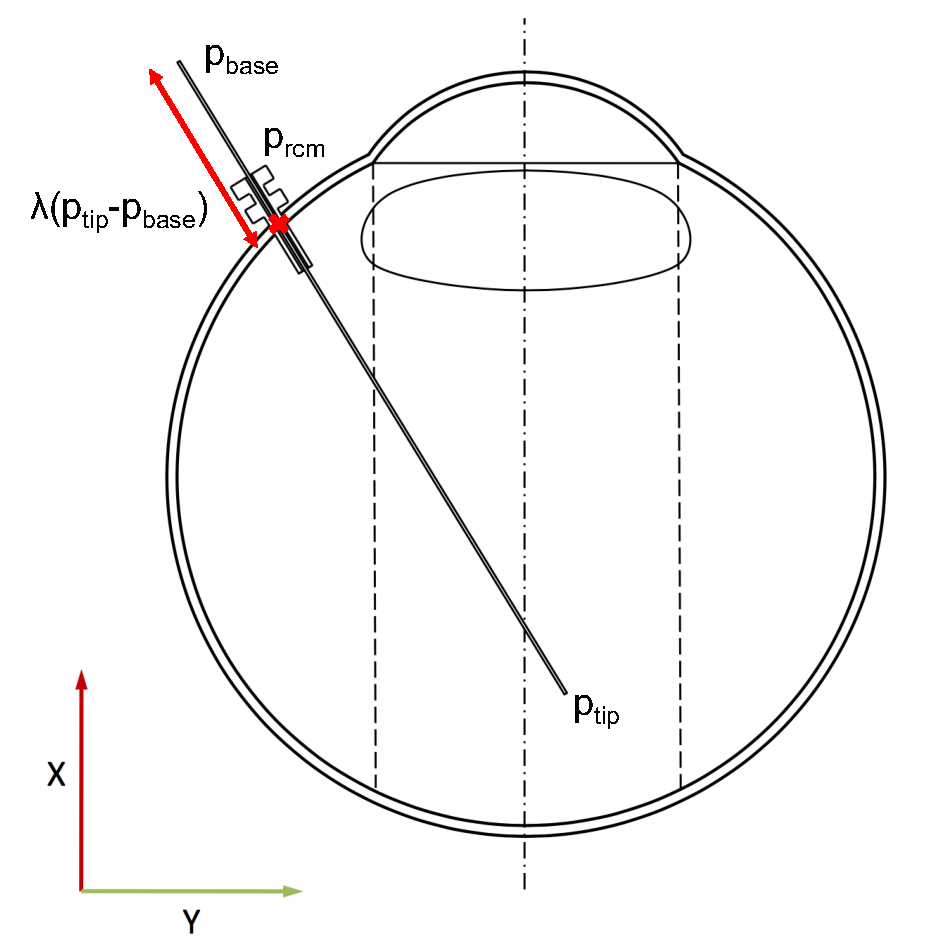
\includegraphics[width=120pt]{lambda}
		\import{images/}{lambda_refactored_tex.pdf_tex}
		\caption{Location of $\bm{p}_{rcm}$}
		\label{lambda}
	\end{center}
\end{figure}

Differentiating with respect to time:
\begin{eqnarray}
	\bm{\dot{p}}_{rcm} = \bm{\dot{p}}_{base}+\lambda(\bm{\dot{p}}_{tip} - \bm{\dot{p}}_{base})+\dot{\lambda}(\bm{p}_{tip} - \bm{p}_{base})
\end{eqnarray}

As previously established, the change in position of any link $i$ can be described as $p_i = J_i q_i$ and thus:
\begin{eqnarray}
	\bm{\dot{p}}_{rcm}=J_{base}\bm{\dot{\theta}}+\lambda(J_{tip}\bm{\dot{\theta}}-J_{base}\bm{\dot{\theta}})+\dot{\lambda}(\bm{p}_{tip}-\bm{p}_{base}) \; ,
\end{eqnarray}
where $J_{base}$ and $J_{tip}$ are the Jacobian matrices corresponding to point $\bm{p}_{base}$ and $\bm{p}_{tip}$ respectively. $J_{tip}$ describes the linear velocity of the tool tip, disregarding the rotation around its own axis ($q_5$). Hence, $J_{tip}$ is equal to the top three rows of $J_0^5$ calculated in the previous section. The points $\bm{p}_{tip}$ and $\bm{p}_{base}$ are on the same rigid link, only at a different distances to he previous joint. Thus, $J_{tip}$ can be modified to describe the motion of point $\bm{p}_{base}$ by substituting $l_6$ with 0, yielding $J_{base}$.
$\bm{\dot{p}}_{rcm}$ can be expressed in matrix form as: 
\begin{eqnarray}
	\bm{\dot{p}}_{rcm} =
		\begin{bmatrix}
			J_{base}+\lambda(J_{tip}-J_{base}) \\[2pt]
			\bm{p}_{tip} - \bm{p}_{base}
		\end{bmatrix}^T
		\begin{bmatrix}
			\bm{\dot{\theta}} \\[2pt]
			\dot{\lambda}
		\end{bmatrix}
	= J_{c}
		\begin{bmatrix}
			\bm{\dot{\theta}} \\[2pt]
			\dot{\lambda}
		\end{bmatrix} 
	= J_{c} \; \bm{\dot{\theta}}_{ext} \; ,
\end{eqnarray}			
with $\bm{\dot{p}}_{rcm} \in \mathbb{R}^{3\times1}$,  $J_{tip}$, $J_{base} \in \mathbb{R}^{3\times5}$ and $J_{c} \in \mathbb{R}^{3\times6}$. The set of extended joint angles $\bm{\theta}_{ext}$ are given as 
\begin{eqnarray}
	\bm{\dot{\theta}} & = & \{ q_1,... \, , q_5, \lambda \} \; .
\end{eqnarray}
Now we can enforce the remote center of motion constraint by setting the velocity of the RCM point to zero. That is, $\bm{p}_{rcm}$ should not change its position.
\begin{eqnarray}
	\bm{\dot{p}}_{rcm}	= J_{c}
			\begin{bmatrix}
				\bm{\dot{q}} \\[2pt]
				\dot{\lambda}
			\end{bmatrix}
					= 0^{3\times 1}
\end{eqnarray}

Hence we have defined the additional kinematic task $\bm{\Phi} = \{x_{rcm}, y_{rcm}, z_{rcm}\}$ and its associated Jacobian $J_c$ in Cartesian coordinates with respect to the robot base frame. 
Although forcing $\bm{\dot{p}}_{rcm}$ to be zero is a constraint of dimension three, modelling the variation of $\lambda$ increases the degrees of freedom by one. Hence, $r=2$ degrees of freedom are lost due to the RCM constraint and $m=3$ degrees of freedom remain to place the tool tip within the eye. 
We choose a set of variables $\bm{Y}$ to represent the position of the end effector that doesn't introduce algorithmic singularities. 
\begin{eqnarray}
	\bm{Y} &=&	\{ x, \phi, \psi\} \; ,
\end{eqnarray}
where $x$ is the global x-position of the tool tip and $\phi$ and $\psi$ describe the angle of the tool.
$\bm{Y}$ and $\bm{\Phi}$ can now be combined to form a set of generalized kinematic functions for the end effector performing the extended task,
\begin{eqnarray}
	\bm{X}_{ext} &=& \{x, \phi, \psi, x_{rcm}, y_{rcm}, z_{rcm} \} \; ,
\end{eqnarray}
and the associated augmented Jacobian
\begin{eqnarray}
	J_{a} =
		\begin{bmatrix}
			J_e \hspace{10pt} 0_{3 \times 1} \\[3pt]
			J_c
		\end{bmatrix}	
		=
		\begin{bmatrix}
			\frac{\partial \bm{Y}}
				{\partial \bm{\theta}} \\[3pt]
			\frac{\partial \bm{\Phi}}
				{\partial \bm{\theta}}
		\end{bmatrix}
\end{eqnarray}
where $J_e$ is the Jacobian matrix relating the end effector x-position and tool angles $\phi $ and $\psi$ to the joint positions. Thus, $J_e$ is composed of the first, fifth, and sixth row of $J_{base} \in \mathbb{R}^{3\times5}$.

Lastly, we need to check if there are any singularities within $J_a$, i.e. if the kinematic functions we chose have any dependencies. One has to differentiate between kinematic and algorithmic singularities. Kinematic singularities refer to any configurations in which $J_e$ is rank deficient, e.g. when two links joined by a revolute joint become co-linear. It was previously established that this is not possible due to the mechanical design of the robot. Algorithmic singularities are introduces by the choice of the kinematic functions $\bm{\Phi}$, if $J_c$ in itself is rank-dependent or if two rows of $J_e $ and $J_c$ are linearly dependent. For the presented case the determinant
\begin{eqnarray}
	det(J_a) &=&	-l_6\cos(q_1)^2\cos(q_3)^2\sin(q_1) \; ,
\end{eqnarray}
is only zero for $q_3 = \pm\frac{\pi}{2}$, which is not a reachable configuration. $J_a$ is listed as Eqn. \ref{J_a_full} in the Appendix.\\

\section{Controller Design}

Having established the augmented Jacobian matrix we can now compute the change in joint position necessary to achieve a certain change in end effector position. However, iteratively using $\Delta \bm{\theta}=J^{\dagger}\Delta \bm{x}$ often does not result in a smooth trajectory from the current to the target pose. If for example the target pose differs from the current pose in only one angle, the Jacobian matrix will return a vector Q correcting the error in angle by rotating the needle. in the next iteration the angle will be right but the RCM point will have shifted and the Jacobian matrix will return a vector Q that translates the needle back. This causes the needle to oscillate until all entries in the current pose are sufficiently close to the target pose. There are two possible solutions to this problen: Either reduce the step size so that the oscillation is very small compared to the overall error in the pose, or introduce a set of weights to determine how fast a parameter should converge. This is done by using the matrix $K$ that multiplies the values in $\Delta \bm{x}$ such that:
\begin{eqnarray}\label{K_J}
	\Delta \bm{\theta}&=&J^{\dagger}\bm{K}\Delta \bm{x}
\end{eqnarray}
where $K \in \mathbb{R}^{6\times6}$ is a diagonal, positive matrix that carries the weights for each entry in $\Delta\bm{x}$. 
Choosing good parameters for $K$ is challenging because of the interdependence of the entries in  $\Delta \bm{x}$. A possible choice for $K$ is presented in Section \ref{K}.

\section{Control Loop}\label{control}

Algorithm \ref{alg:control_loop} shows the control loop that implements Eqn. \ref{K_J} in order to perform a small step from the current position to a target position. It is implemented in a MATLAB script that can receive the positions of simulation objects and returns the updated values for the joint angles and $\lambda$ calculated by the Jaobian matrix.

\begin{algorithm}
  \begin{algorithmic}[1]
 \STATE $\text{current\_pose} \leftarrow \textit{get\_task\_pose}()$
 \WHILE {$max(abs(\text{target\_pose}-\text{current\_pose}))>0.0002$}
  \STATE $\text{error} \leftarrow \text{target\_pose}-\text{current\_pose}$
  \STATE $\text{joint\_positions}=\textit{get\_joint\_positions}()$
  \STATE $\bm{Q} \leftarrow \textit{L\_to\_Q}(\text{joint\_positions})$
  \STATE $[\Delta \bm{Q},\Delta\lambda] \leftarrow J_a(\bm{Q},\bm{\lambda})^{-1}\bm{K} \; \text{error}$
  \STATE $\Delta L \leftarrow \textit{Q\_to\_L}(\Delta \bm{Q})$
  \STATE $\textit{set\_joint\_positions}(\text{joint\_positions}+\Delta \bm{L})$
  \STATE $\bm{\lambda} \leftarrow \bm{\lambda} + \Delta\bm{\lambda}$
  \STATE $\textit{move\_RCM}(\bm{\lambda})$
  \STATE $\text{current\_pose} \leftarrow \textit{get\_task\_pose}()$
 \ENDWHILE 
  \end{algorithmic}
  \caption{$\text{Control\_Loop}(\bm{K}, \text{target\_pose},J_a,\lambda)$} \label{alg:control_loop}
\end{algorithm}

In each iteration of the main body, the error between current and target pose is computed. The current slider positions $L$ are obtained from the simulation and converted to the set of simplified joint variables $q_i$. The augmented Jacobian matrix is computed using $\lambda$ and the current joint positions, multiplied with the control matrix $K$ and the error to obtain update values both for the simplified joint variables $q_i$ as well as $\lambda$. The joint variables are converted back to a set of slider displacements and returned to the simulation. the RCM point in the simulation model is moved according to $\Delta\lambda$ and the new current task pose $\bm{X}_{ext} = \{x, \phi, \psi, x_{rcm}, y_{rcm}, z_{rcm}\}$ is obtained. The main body of the control loop is executed until the current pose is sufficiently close to the target pose (ensuring the position of the RCM is within a bounded accuracy).

\section{Measuring the Accuracy of the RCM position}\label{Setup}

In order to compare the precision of the augmented Jacobian matrix, a series of constrained movements of the needle within the eye is performed. Figure \ref{injection_illustration} illustrates the sequence of points the needle tip should follow.

\begin{figure}[h!]
	%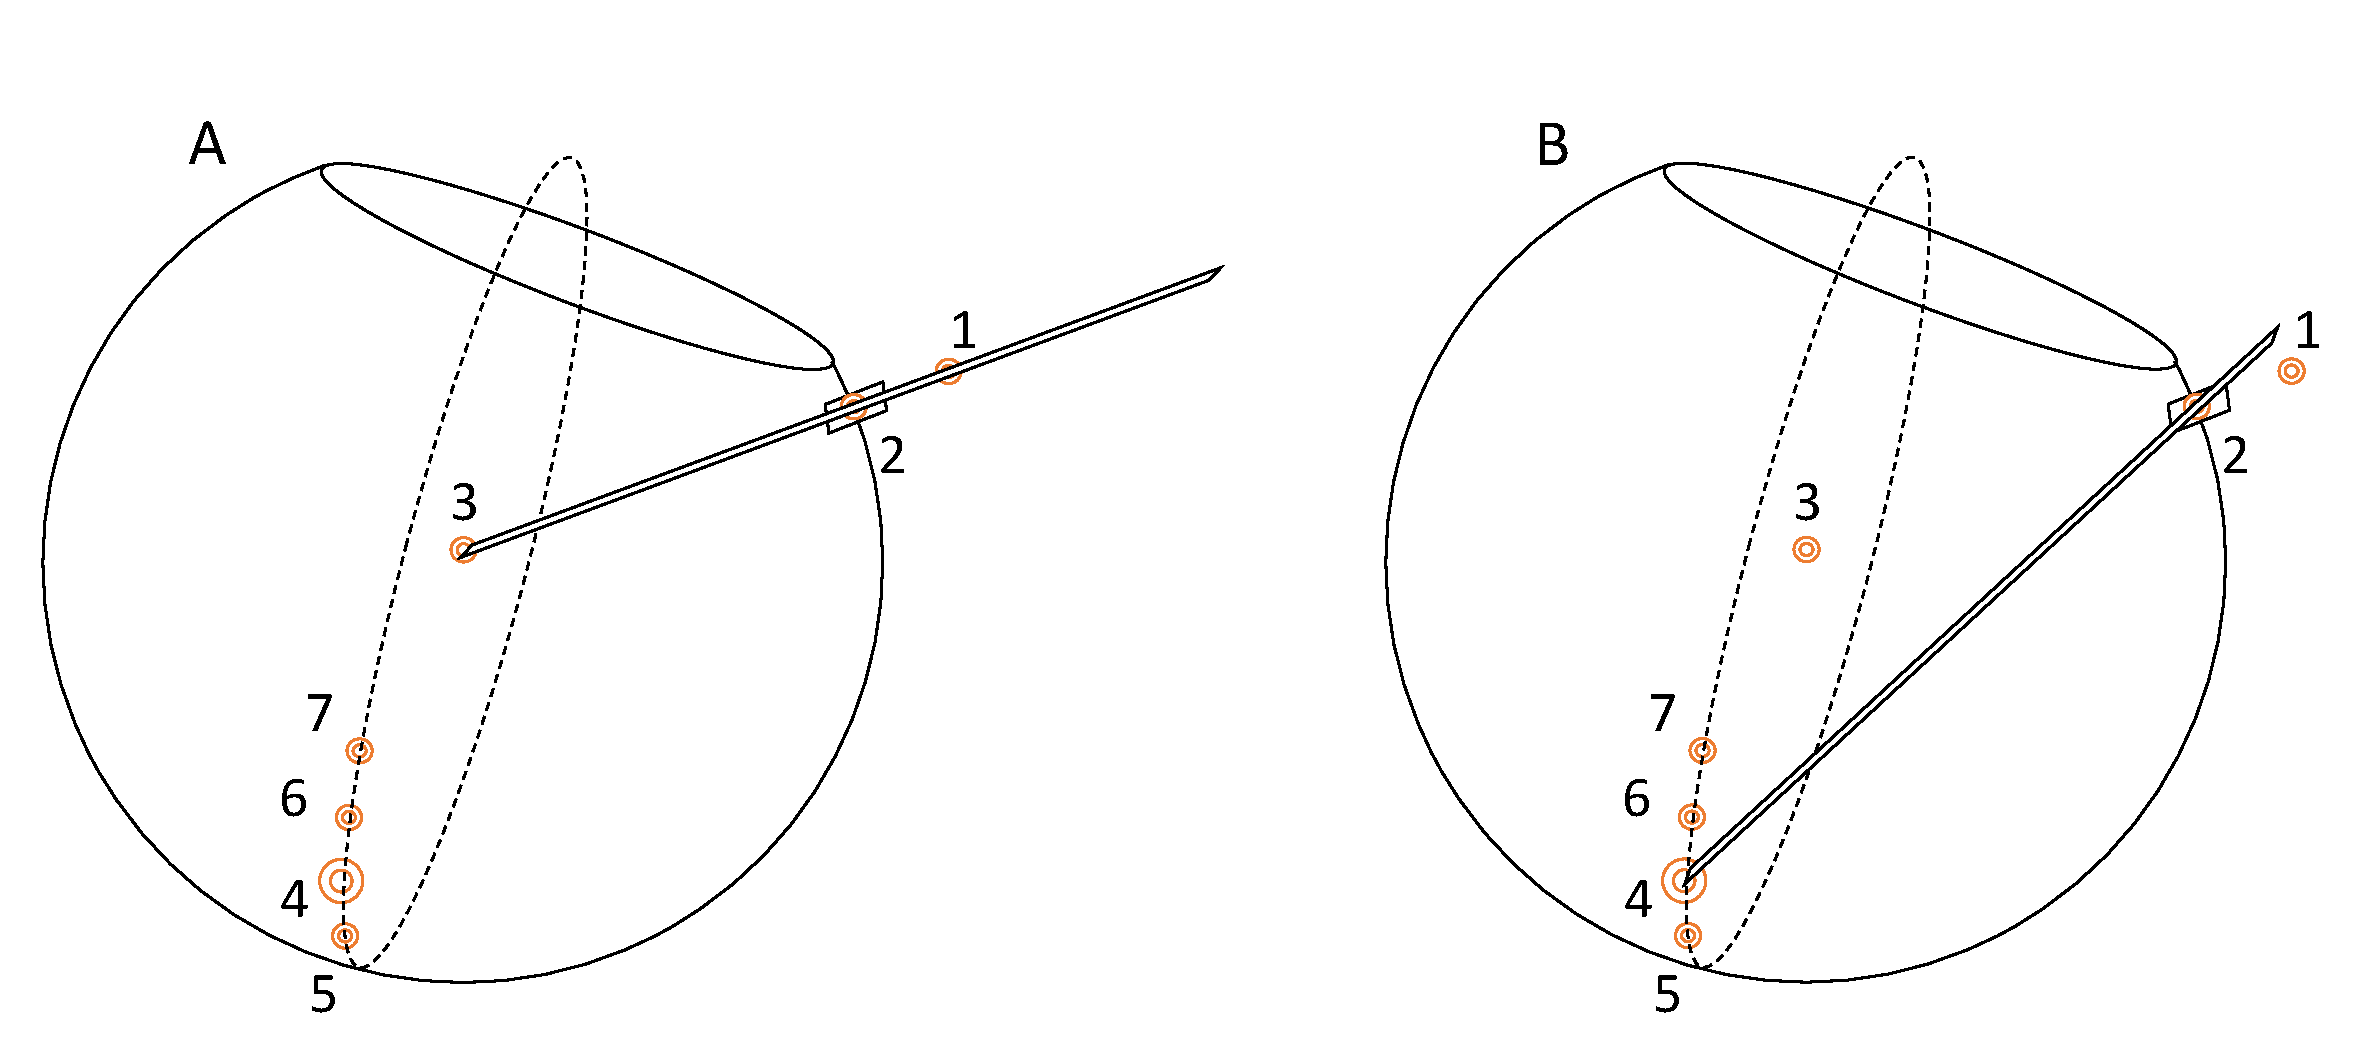
\includegraphics[width=400pt]{injection_illustration}
	\import{images/}{injection_illustration_refactored_tex.pdf_tex}\caption{Setup for measuring the precision of the RCM point. \textbf{A}: The needle enters the eye through the trocar until it reaches point \textbf{3}. \textbf{B}: The needle tip moves from point \textbf{3} to points \textbf{4}-\textbf{7} while keeping the RCM point, located at \textbf{2}, steady.}
	\label{injection_illustration}
\end{figure}

Injection begins by moving the tool tip from an arbitrary point outside the eye to position \textbf{2} via unconstrained movement. Once point \textbf{2} is reached, the RCM point will be positioned at the tip of the needle ($\lambda=1$) and control via the augmented Jacobian begins. The tool is pivoted around its tip until point \textbf{1} lies on the needle, and thus the needle is aligned with the trocar. The needle is then moved forwards in a straight line until its tip reaches point \textbf{3}. From there, points \textbf{4}-\textbf{7} located on the inner surface of the eye will be visited, returning to position \textbf{3} each time.

\section{Modelling the Surgical Robot in V-REP}

This section describes the process of generating two Simulation models that can be controlled via the MATLAB remote API from the CAD data of the robot: One model for use in forwards kinematics mode, where the slider positions $L_i$ are controlled via a MATLAB script according to the values computed by the Jacobian matrix, and one model for use in inverse kinematics mode, where only the target positions for the needle tip and the RCM are controlled by the MATLAB script and the joints are controlled by the internal IK solver.

The CAD model of the robot is first imported into V-REP as a single triangle mesh. Using the automatic mesh subdivision, a new shape is generated for all elements that are not connected via a common edge and thus, all components of the robot are extracted as separate rigid links. Now, joint objects are added to specify the movement of the links relative to each other. Figure \ref{vrep_model} shows the finished model of the robot.  

\begin{figure}[b!]
	\centering
	%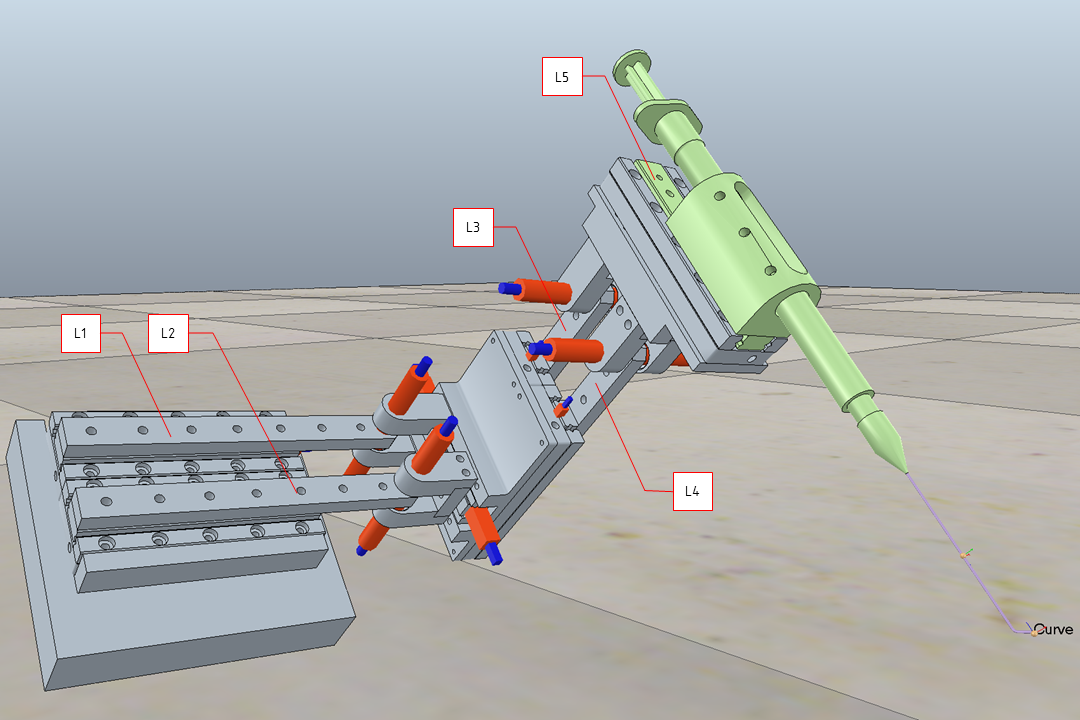
\includegraphics[width=300pt]{vrep_model}
	\import{images/}{vrep_model_1_tex.pdf_tex}
	\caption{The surgical robot modelled in V-Rep}
	\label{vrep_model}
\end{figure}

Next, we need to specify how the different links and joints are connected with each other. In the real robot, a PCJM consists of two sliders contribute that to the translation and rotation of a subsequent stage. This cannot be directly modelled in V-REP because each element (e.g. the middle stage) can only have one parent object (i.e. one of the sliders in the PCJM). To assemble the robot model into a single kinematic chain in which every object has only one parent element, we first connect the robot base plate with the needle via one slider of each PCJM (corresponding to $L_2$ and $L_4$). From the needle, we make our way back down towards the middle plate using slider $L_3$ and from the middle pate to the base plate via slider $L_1$. Since this second pair of sliders $L_3$ and $L_1$ is now "dangling" from their respective target plate (indicated by a green overlay in Figure \ref{vrep_hierarchy}) we need to inform the simulation that the two sliders should be connected to their respective base plates. Therefore, two sets of tip-target pairs are introduced. For each pair, one dummy is attached to the slider and one to the corresponding base plate and both are constrained to overlap in position and orientation (indicated by blue dotted arrows in Figure \ref{vrep_hierarchy}).     

\begin{figure}[t!]
	\centering
	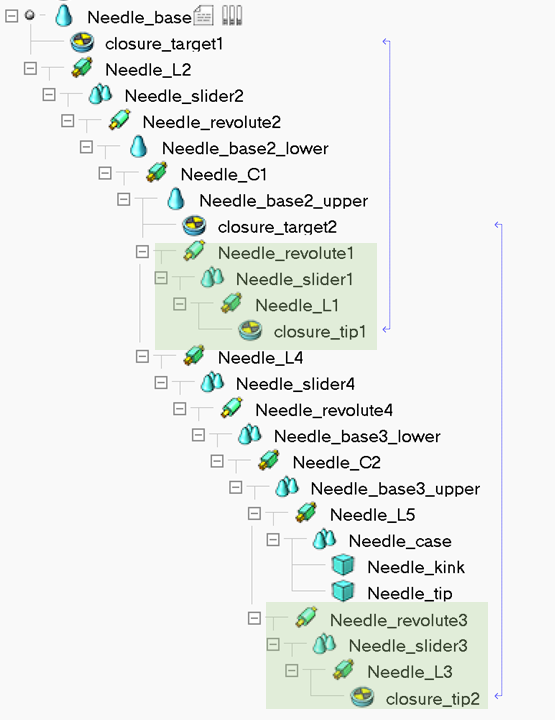
\includegraphics[width=8cm]{vrep_hierarchy}
	\caption{The scene hierarchy for the finished robot model. The green boxes indicate the sidearms of the kinematic chain that need to be constrained to be connected to their respective base plate via a tip-target pair (blue arrows).}
	\label{vrep_hierarchy}
\end{figure}

Until now, the modelling process has been the same for the forwards and inverse kinematics model. If we want to control the robot in forwards kinematics mode, the five prismatic joints corresponding to the stick-slip piezo actuators are set to "Force/Torque" mode and all other joints are set to "passive mode", meaning that they will not be actuated but can be passively rotated or displaced by connected moving links. For the inverse kinematics model, \textbf{all} joints are put into inverse kinematics mode so they can be controlled by the inverse kinematics solver. Additionally, we need to define the inverse kinematic task for the robot, described in the next section.

\subsection{Defining the Inverse Kinematic Task}

\begin{figure}[h!]
	\import{images/}{IK_refactored_2.pdf_tex}
	\caption{Schematic overview of the kinematic chain in V-REP. Objects connected by a bold black arrow indicate the primary kinematic chain which corresponds to the simplified serial robot in \ref{Manipulator}. Objects within a grey box belong to the same stage of the robot, i.e. one of the PCJMs or the final prismatic stage. A total of 4 IK pairs illustrated by yellow rings constrain (1) the position of the needle tip (2) the position of the RCM and (3,4) the position of the second slider within each PCJM}
	\label{IK_chain}
\end{figure}

Figure \ref{IK_chain} shows the kinematic chain used to define the inverse kinematics task. Since the robot consists of subsequent PCJMs, it cannot be modelled as a linear kinematic chain (every element can only have one parent in the scene hierarchy). Instead, three distinct IK groups that are defined. The first IK group governs the position of both the tool tip and the RCM point by finding a joint configuration that minimizes the distance to their respective targets. The tip and RCM position need to be included in the same IK group since they are on the same rigid link and in a way represent conflicting goals for the needle pose between which a compromise needs to be found. The other two IK groups are used to 'close the loop', that is to connect the side chains to their respective bottom plates. The two loop-closure IK tasks are added solely for cosmetic reasons, since even without them the position of the second slider in each PCJM could be uniquely reconstructed from the position of the first slider and the angle of the subsequent revolute joint.